\section{Optical properties of the sphere }
\label{sec:opt}

The LXe target bubble should not be too large in order to avoid double scatters. 
The HPFS shell should be large enough to reduce internal reflections, but not 
too large which would attenuate the scintillation light. The material of the 
shell should have a refractive index as similar to LXe as possible in order to 
have minimal diffraction from the original direction of the photons when they 
travel from the LXe target to the sphere. Corning HPFS 8655 is chosen as the shell 
material. The refractive index of HPFS 8655 is 1.575 at 185 nm (LXe R.I. 1.61). 
In Fig.~\ref{fig:hpfsRIcalibration} (left panel), are the refractive indexes at various wavelengths 
as provided on the HPFS 8655 fact sheet as well as a naive extrapolation to lower wavelengths 
which are relevant to us. 

\begin{figure}[h]
   \centering
   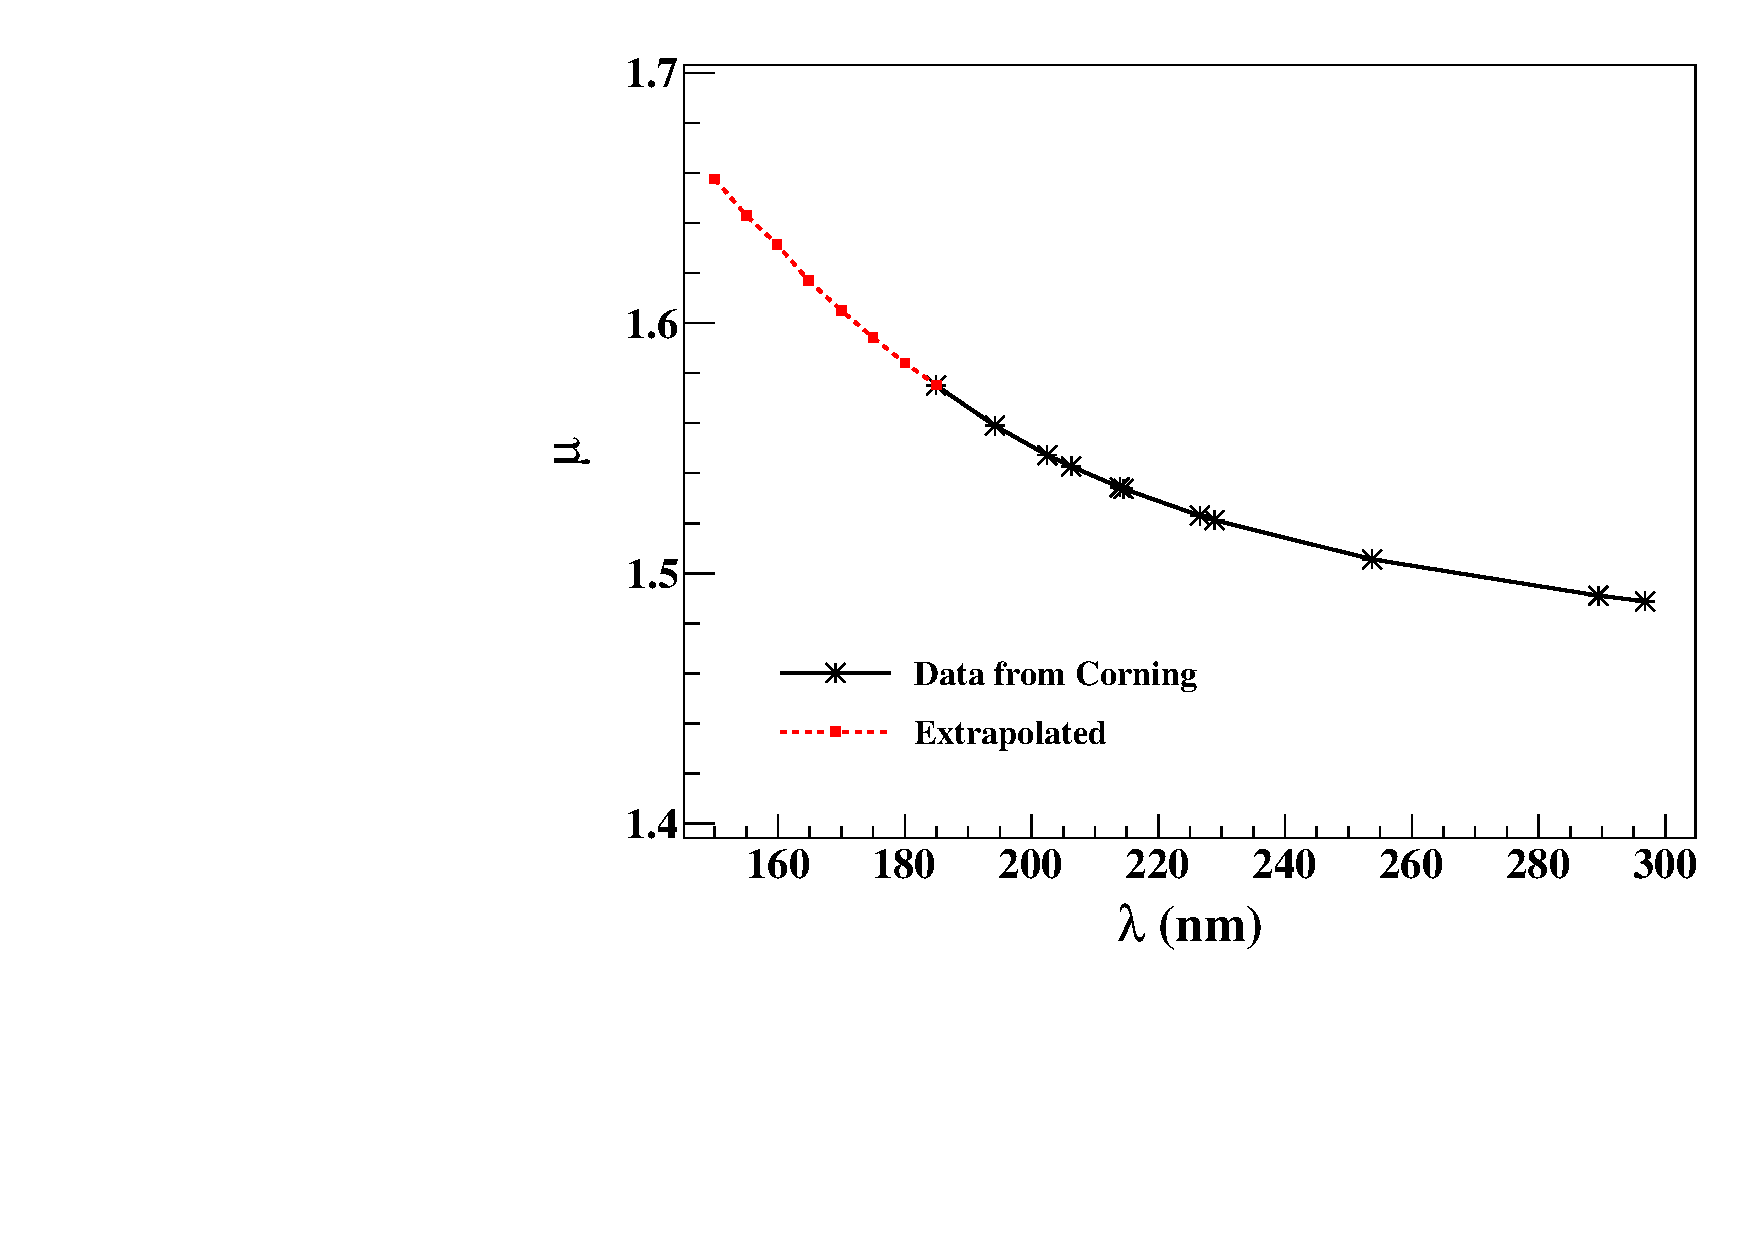
\includegraphics[width=0.48\textwidth]{RI-calibration.pdf}
    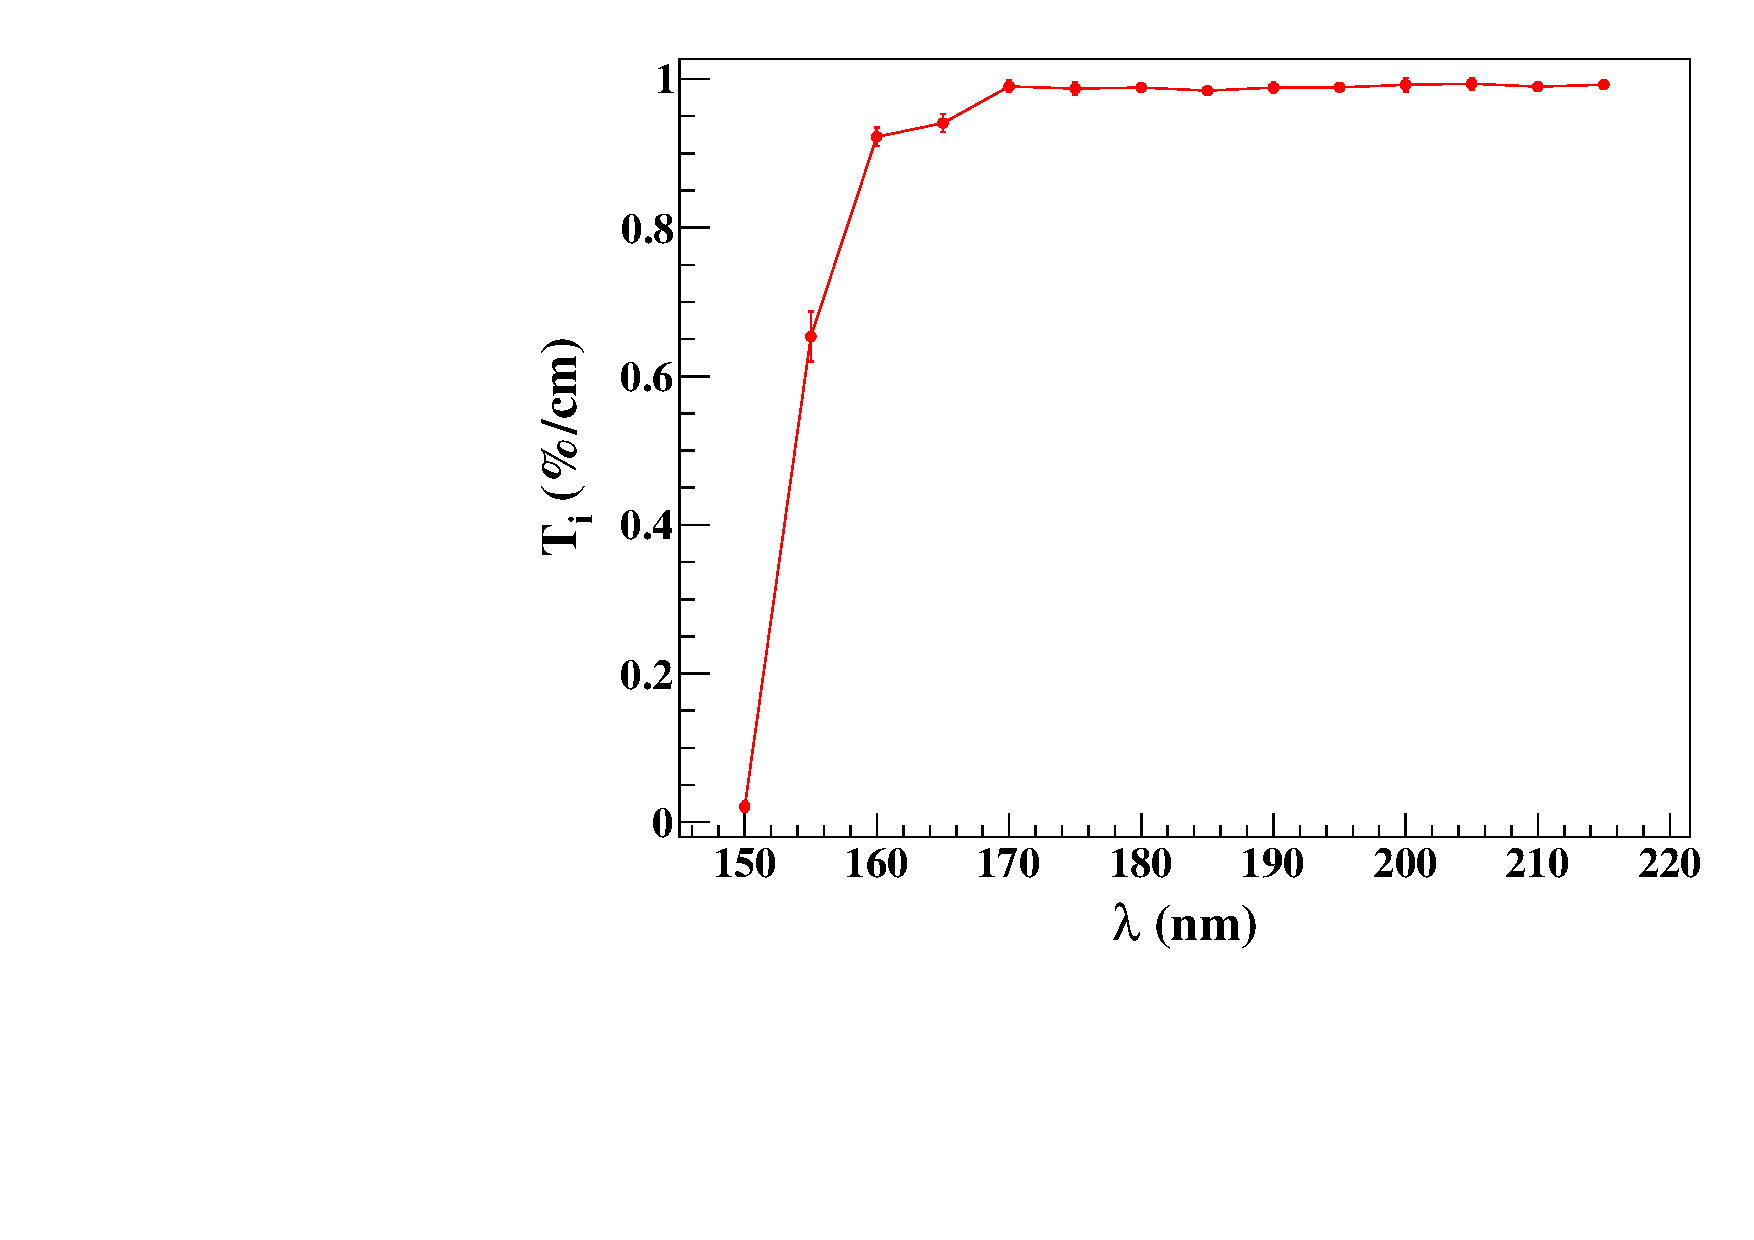
\includegraphics[width=0.48\textwidth]{IntTransmittance.pdf}
   \caption{The important characteristics of HPFS-8655. (Left) The refractive index as provided by corning and 
   extrapolated to relevant wavelength range. (Right) The internal transmittance ($T_{i}$).} 
   \label{fig:hpfsRIcalibration}
\end{figure}

The transmittance of the material is an extremely crucial parameter to optimize the 
dimension of the shell. Therefore, a sample of HPFS 8655 was tested for transmittance 
using a VUV monochromator. 
In fig.~\ref{fig:hpfsRIcalibration} (right panel), the measured 
transmittances (\%/cm) at (150 - 215)~\,nm are plotted. At 175~\,nm, the intrinsic transmittance 
of the sample about 98.7\%/cm.  


The dimension of the fused silica shell is optimized by studying the path of the 
scintillation photons using a GEANT4 based simulation~\cite{AGOSTINELLI2003250}. 
The sources that will be used for exciting the xenon, and creating the supperradiance 
(signal) as well as the standard emission (background), will be $^{137} \mathrm{Cs}$ 
(662 keV) and $^{57} \mathrm{Co}$(122keV \& 136 keV) for ER and $^{241}$AmBe , 
D-D neutron generator, or neutron produced in an accelerator for NR . The mean 
free path for this energy is a couple of mm ($^{57} \mathrm{Co}$) and (0.5 - 3) 
cm ($^{137} Cs$).  The outer radius of the shell is 3 cm, while the inner radius of the 
hollow space that holds the LXe is 1 cm. 


